\documentclass[11pt]{article}

\usepackage[letterpaper, margin=1in]{geometry}
\usepackage{listings}
\usepackage[spanish]{babel}
\usepackage[utf8]{inputenc}
\usepackage{multirow}
\usepackage{tabularx}
\usepackage{longtable}



%Figuras
\usepackage{graphicx, subfigure}
\usepackage[]{tikz}
\usepackage{pbox}

%Matemática
\usepackage{amsmath}
\usepackage{amssymb}

%Símbolos mate extra (alfabetos, etc.)
\usepackage{mathrsfs}


%Algoritmos
\usepackage{float}
\usepackage{algorithm}
\usepackage{algorithmicx}
\usepackage{algpseudocode}
\usepackage{listings}


\usepackage{color}
\usepackage{hyperref}

\usepackage{mdframed}
\usepackage{tcolorbox}
\usepackage{multicol}
\usepackage{booktabs}
\usepackage{tabulary}
\definecolor{darkblue}{rgb}{0 , 0.054 , 0.196}



\title{Reporte de Laboratorio 3}
\author{Emmanuel - B51296}

\begin{document}

\maketitle
\hrule
\hrule
\tableofcontents
\hspace{5mm}
\hrule
\hrule


\section{Introducción}
Este laboratorio tuvo como objetivo aprender sobre la creación de clases emplantilladas, así como ampliar los conocimientos de sobrecarga de operadores
\subsection{Objetivos}
\begin{itemize}
	\item Aprender acerca de la construcción de clases emplantilladas en C++.
	\item Aprender sobre sobrecarga de operadores en C++.
\end{itemize}

\section{Código}

\subsection{Figura.h}
\begin{lstlisting}
#ifndef FIGURA_H
#define FIGURA_H
#include <iostream>
#include "string"
#include <math.h> 

using namespace std;

class Figura{
public:
string color;
string nombre;
Figura();
Figura(string nombre, string color);
virtual double area();
virtual double perimetro();
virtual ~Figura();
double papa();

};
#endif /* FIGURA_H */

\end{lstlisting}

\subsection{Figura.cpp}
\begin{lstlisting}
#include "Figura.h"

///Constructor de la clase figura.
Figura::Figura(){
}
///Desstructor de la clase figura.
Figura::~Figura(){
}

///Constructor sobrecargado de la clase figura
Figura::Figura(string nombre, string color){
this-> nombre = nombre;
this-> color = color;
}
///Funcion general para calculo de area de una figura.
double Figura::area(){
cout << "Implementar en subclases de figuras" << endl;
return 0;
}
///Funcion general para calculo de perimetro de una figura.

double Figura::perimetro(){
cout << "Implementar en subclases de figuras" << endl;
return 0;
}


\end{lstlisting}

\subsection{Triangulo.h}
\begin{lstlisting}
#ifndef TRIANGULO_H
#define TRIANGULO_H
#include <iostream>
#include "string"
#include "Figura.h"
#include <math.h> 



using namespace std;

class Triangulo : public Figura{
public:
string color;
string nombre;
void operator~();
void operator!();
double l1;
double l2;
double l3;
double s;
Triangulo();
Triangulo(string nombre, string color, double l1, double l2, double l3);
virtual double area();
virtual double perimetro();
virtual ~Triangulo();
};
#endif /* TRIANGULO_H */
\end{lstlisting}

\subsection{Triangulo.cpp}
\begin{lstlisting}
#include "Triangulo.h"
#include "Figura.h"

///Constructor de la clase triangulo.
Triangulo::Triangulo(){
}
///Destructor de la clase derivada triangulo.
Triangulo::~Triangulo(){
}
///Constructor sobrecargado de la clase derivada triangulo.
Triangulo::Triangulo(string nombre, string color, double l1, double l2, double l3){
this-> nombre = nombre;
this-> color = color;
this-> l1= l1;
this-> l2= l2;
this-> l3= l3;
this-> s= (l1+l2+l3)/2;

}

///Funcion general para calculo de area de un triangulo.
double Triangulo::area(){
double sp = this->s;
double la1 = this-> l1;
double la2 = this-> l2;
double la3 = this-> l3;
double a= sqrt(sp*(sp-la1)*(sp-la2)*(sp-la3));
return a;
}

///Funcion general para calculo de perimetro de un triangulo.
double Triangulo::perimetro(){
double p;
p = this-> l1 + this-> l2 + this-> l3;
return p;
}

///Desplegador de los datos generales del triangulo.
void Triangulo::operator~(){
cout << "Nombre: " << this-> nombre <<endl;
cout << "Color: " << this-> color <<endl;
cout << "Longitud de los lados " << this-> l1 << ", " << this-> l2 << ", " << this-> l3 <<endl;
cout<< "\n" << endl;

}
///Desplegador del area y el perimetro del triangulo.
void Triangulo::operator!(){
cout << "Area: " << this-> area() <<endl;
cout << "Perimetro: " << this-> perimetro() <<endl;
cout<< "\n" << endl;

}

\end{lstlisting}

\subsection{Cuadrado.h}
\begin{lstlisting}
#ifndef CIRCULO_H
#define CIRCULO_H
#include <iostream>
#include "string"
#include "Figura.h"
#include <math.h> 



using namespace std;

class Circulo : public Figura{
public:
string color;
string nombre;
void operator~();
void operator!();
double r;
Circulo();
Circulo(string nombre, string color, double r);
virtual double area();
virtual double perimetro();
virtual ~Circulo();
};
#endif /* CIRCULO_H */

\end{lstlisting}

\subsection{Cuadrado.cpp}
\begin{lstlisting}
#include "Figura.h"
#include "Cuadrado.h"

const double PI  =3.141592653589793238463;
///Constructor de la clase cuadrado.
Cuadrado::Cuadrado(){
}
///Destructor de la clase derivada cuadrado.
Cuadrado::~Cuadrado(){
}
///Constructor sobrecargado de la clase derivada cuadrado.
Cuadrado::Cuadrado(string nombre, string color, double l){
this-> nombre = nombre;
this-> color = color;
this-> l=l;

}

///Funcion general para calculo de area de un cuadrado.
double Cuadrado::area(){
double a = pow(this-> l, 2);
return a;
}

///Funcion general para calculo de perimetro de un cuadrado.
double Cuadrado::perimetro(){
double p;
p = 4*this->l;
return p;
}

///Desplegador de los datos generales del cuadrado.
void Cuadrado::operator~(){
cout << "Nombre: " << this-> nombre <<endl;
cout << "Color: " << this-> color <<endl;
cout << "Longitud del lado " << l <<endl;
cout<< "\n" << endl;
}

///Desplegador del area y el perimetro del cuadrado.
void Cuadrado::operator!(){
cout << "Area: " << this-> area() <<endl;
cout << "Perimetro: " << this-> perimetro() <<endl;
cout<< "\n" << endl;

}

\end{lstlisting}

\subsection{Circulo.h}
\begin{lstlisting}
#ifndef CIRCULO_H
#define CIRCULO_H
#include <iostream>
#include "string"
#include "Figura.h"
#include <math.h> 



using namespace std;

class Circulo : public Figura{
public:
string color;
string nombre;
void operator~();
void operator!();
double r;
Circulo();
Circulo(string nombre, string color, double r);
virtual double area();
virtual double perimetro();
virtual ~Circulo();
};
#endif /* CIRCULO_H */

\end{lstlisting}

\subsection{Circulo.cpp}
\begin{lstlisting}
#include "Figura.h"
#include "Circulo.h"

const double PI  =3.141592653589793238463;
///Constructor de la clase circulo.
Circulo::Circulo(){
}
///Destructor de la clase derivada circulo.
Circulo::~Circulo(){
}
///Constructor sobrecargado de la clase derivada circulo.
Circulo::Circulo(string nombre, string color, double r){
this-> nombre = nombre;
this-> color = color;
this-> r=r;

}

///Funcion general para calculo de area de un circulo.
double Circulo::area(){
double a = PI*pow(this-> r, 2);
return a;
}

///Funcioon general para calculo de perimetro de un circulo.
double Circulo::perimetro(){
double p;
p = 2*PI*this->r;
return p;
}

///Desplegador de los datos generales del circulo.
void Circulo::operator~(){
cout << "Nombre: " << this-> nombre <<endl;
cout << "Color: " << this-> color <<endl;
cout << "Longitud del radio " << r <<endl;
cout<< "\n" << endl;

}

///Desplegador del area y el perimetro del circulo.
void Circulo::operator!(){
cout << "Area: " << this-> area() <<endl;
cout << "Perimetro: " << this-> perimetro() <<endl;
cout<< "\n" << endl;

}

\end{lstlisting}

\section{Diagrama UML}
\begin{figure}[!ht]
	\caption{Diagrama UML de la clase figura}
	\centering
	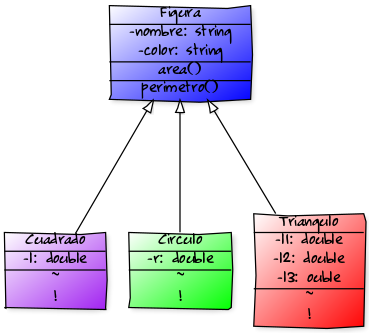
\includegraphics[width=0.5\textwidth]{UML}
\end{figure}


\section{Conclusiones}
Durante este laboratorio se aprendió sobre la importancia del manejo de las clases y sus diferentes opciones en funcionalidad, para crear programas complejos utilizando las diversas características que las clases ofrecen, como polimorfismo y herencia. De igual forma, se aprendió sobre la utilidad de la sobrecarga de operadores, para simplificar el uso de ciertas funciones en una clase en específico.




\end{document}
